%======================================================================
%----------------------------------------------------------------------
%               XX                              X
%                                               X
%               XX    XXX   XXX   XXX      XXX  X  XXXX
%                X   X   X X   X X   X    X   X X X
%                X   XXXXX XXXXX XXXXX    X     X  XXX
%                X   X     X     X     XX X   X X     X
%               XXX   XXX   XXX   XXX  XX  XXX  X XXXX
%----------------------------------------------------------------------
%  	         A SKELETON FILE FOR IEEE PAPER GENERATION
%----------------------------------------------------------------------
%======================================================================

% first, uncomment the desired options:
\documentclass[%
				10pt,
        %draft,
        %submission,
        %compressed,
        final,
        %
        %technote,
        %internal,
        %submitted,
        %inpress,
        %reprint,
        %
        %titlepage,
        notitlepage,
        %anonymous,
        narroweqnarray,
        inline,
        twoside,
        ]{ieee}
%
% some standard modes are:
%
% \documentclass[draft,narroweqnarray,inline]{ieee}
% \documentclass[submission,anonymous,narroweqnarray,inline]{ieee}
% \documentclass[final,narroweqnarray,inline]{ieee}

% Use the `endfloat' package to move figures and tables to the end
% of the paper. Useful for `submission' mode.
%\usepackage {endfloat}

% Use the `times' package to use Helvetica and Times-Roman fonts
% instead of the standard Computer Modern fonts. Useful for the 
% IEEE Computer Society transactions.
% (Note: If you have the commercial package `mathtime,' it is much
% better, but the `times' package works too).
%\usepackage {times}

% In order to use the figure-defining commands in ieeefig.sty...
\usepackage{ieeefig}

% Added Margins
\usepackage[left=1.5in, right=1.5in, top=1.0in, bottom=1.0in]{geometry}
\usepackage{layout}

\begin{document}

%----------------------------------------------------------------------
% Title Information, Abstract and Keywords
%----------------------------------------------------------------------
\title[Reputation Management with Distributed Brokers]{%
       Reputation Management  in Peer to Peer Cloud Storage Utilizing Virtual Currency Exchange and Distributed Brokers}

% format author this way for journal articles.
%\author[SHORT NAMES]{%
%      Bryan Olivas\member{Student Member}
%      \authorinfo{%
%      A. Author is with the Department of Electrical Engineering,
%      Some University, Somewhere CA, 90210, USA,
%      Phone: \mbox{(xxx) xxx-xxxx}, email: \mbox{xxx@xxxx.xxx.xxx}}
%    \and
%      Jiawei Li\member{Student Member}
%      \authorinfo{%
%      B. Author is with the Department of Electrical Engineering...}
%    \and
%      and Vance Thornton\member{Student Member}
%      \authorinfo{...}
%  }

% format author this way for conference proceedings
\author{%
      Bryan Olivas
    \and
      Jiawei Li
    \and
      and Vance Thornton
}

% specifiy the journal name
%\journal{IEEE Transactions on Something, 1997}

% Or, when the paper is a preprint, try this...
%\journal{IEEE Transactions on Something, 1997, TN\#9999.}

% Or, specify the conference place and date.
%\confplacedate{Ottawa, Canada, May 19--21, 1997}

% make the title
\maketitle               

% do the abstract
\begin{abstract}
Virtual currency is a powerful tool for encouraging cooperation in a peer to peer cloud storage service.  In this paper we present a design for a P2P storage system which utilizes a virtual currency for reputation management and compare it to existing currency based P2P reputation management systems.  Our system offers several advantages over existing systems.  One of the most significant of these is that we utilize a distributed broker to help ensure that the nodes participating in a data transfer transaction fulfill their obligations.  Several types of possible attacks on the system are analyzed and a simulation is used to measure the expected effectiveness of the system.
\end{abstract}

% do the keywords
\begin{keywords}
reputation management, peer-to-peer, virtual currency, distributed broker
\end{keywords}

%----------------------------------------------------------------------
% SECTION I: Introduction
%----------------------------------------------------------------------
\section{Introduction}

\PARstart Data storage and transfer play a significant role in many cloud computing applications.  Cloud storage services such as Amazon S3, while very popular, do not necessarily represent the most desirable model for cloud storage.  One issue with such services is limited transparency.  In many cases the source code for the software that is used to provide the service is not made available to the public and so is not available for wide public verification.  Users of the service must trust that the software is sufficiently bug free and secure.  Another drawback to such services is relatively centralized control over physical infrastructure.  All other things being equal it would be preferable if more than one organization was responsible for providing and protecting this infrastructure.  Users can mitigate this issue by storing their data in multiple storage clouds, but this can entail additional cost and complexity.  The cost associated with data storage and transfer is a significant barrier in many applications.  Using a peer to peer network for cloud data storage can potentially eliminate these issues.  If the software is open source then there is a high degree of transparency and a wide community can participate in the verification of the software.  Peer to peer systems are also highly decentralized.  No single company or individual controls the infrastructure.  Finally if peers are motivated to cooperate the data storage and transfer costs are shared by the peers in a way that can be proportional to the benefit they receive.  Peer to peer cloud storage can make possible applications that would have otherwise been financially infeasible. 

One of the central problems in peer-to-peer systems is ensuring that peers contribute to the system.  For our system design we focus on a virtual currency based approach to this problem.  Virtual currency provides a natural means of tracking the transfer of value between peers.  When a peer provides resources to another peer it receives currency that it can use to acquire resources from other peers.  As with currency in the real world every transaction carries the risk that either the buyer or seller will not provide what was promised.  A broker is an entity that can used to mitigate this risk by acting as a trusted third party that performs the actual exchange on behalf of the buyer and seller.  In this paper we present a design for a peer-to-peer storage system that has brokered virtual currency transactions.  The broker in our system design is distributed to the peers in the network rather than centralized.  This lack of centralization makes the system more robust because a potential single point of failure is eliminated.  Involving more nodes in the broker role also makes the broker more trustworthy.  It is more likely that a single node could be malicious or compromised than that the majority of a large number of nodes would be so.  The use of a broker is particularly well suited to peer-to-peer storage because the broker can utilize hashes and encryption keys to verify and perform the transfer.

%----------------------------------------------------------------------
% SECTION II: Related Work
%----------------------------------------------------------------------
\section{Related Work}

\subsection{Existing Currency-Based P2P Reputation Management Systems}
P2P has experimented with various schemes and incentives in order to persuade nodes into resource cooperation.  Those in the P2P community have identified these as �Incentive-Based Protocols.�  These protocols aim to give incentives or payoffs to nodes in order to make them cooperate ~\cite{gupta}.  The idea is to reward a node with an agreed upon type of credit or virtual currency for their contribution of shared resources.  Some implementations have implored the notion that the reputation of a node is a decaying function of time ~\cite{gupta}.  This would require that a node continuously share resources or provide services.  This can lead to the formation of trust groups.  These can be viewed as trusted communities of nodes.  Each member of a trust group shares the same reputation.  This also means that the individual node store information about every other node in the system.  This, however, may not scale well.  The question remains; how to maintain a fair voluntary resource sharing amongst individual peers.  Currency-based P2P reputation management attempts to solve this.  There are varying factors.  The system must have mechanisms to deal with these factors.  The system needs to manage the challenges of malicious, selfish (rational), altruistic, and free-rider (freeloader) nodes.  The system also must manage the transfer of currency.  We will discuss some of the various systems.  

Dandelion ~\cite{sirivianos} implements P2P static content distribution that relies on security, specifically symmetric cryptography, to provide robust incentives to individual peers.  There exists a server, trusted third party, that maintains a virtual economy.  Each peer has a credit balance.  The server attracts selfish clients by rewarding them with virtual credit for contributing resources.  Inversely the server charges clients for consuming resources from selfish clients.  Transactions are separated into chunks.  If the client has enough virtual credit then that client may acquire a resource chunk.  The system uses encryption and decryption of the data to serve as proof that the exchange has been completed appropriately.  

KARMA ~\cite{vishnumurthy} proposes a framework to avoid freeloaders.  This is accomplished by keeping track of resource contribution and consumption of a given node.  This observation is represented by a scalar value that they call karma.  Nodes are given incentives for contributing resources to a global pool.  The system accounts for the amount of resources that a node has contributed and the amount the node has consumed.  The peer�s standing is stored within a global system.  Groups of nodes serve as a bank-set.  The bank-set is in charge of keeping track of the karma associated to the corresponding peer.  The peer�s balance adjusts accordingly as the peer contributes and consumes resources.  A monetary value is associated with a pre-defined transaction.  A transaction can not proceed if the resource-consumer does not have enough karma than it takes to make payment for the resources involved ~\cite{vishnumurthy}.  This forces all participants to be uniform between resources contributed and consumed.  

Escrow Service, PPay, and WhoPay all employ fair exchange schemes to detect �cheater� peers in the system.  A trusted third party is used to mediate all questionable exchanges.  Peers can and often find loopholes to circumvent certain scenarios.  Dandelion ~\cite{sirivianos} uses a similar scheme, however, the trusted third party mediates all exchanges in order to prevent a client from obtaining a resource without sufficient credit.

\subsection{Payment Schemes}
One of the focus areas of reputation management is defining various incentive schemes for node cooperation.  Although different in implementation all of these schemes promote node collaboration using P2P.

Monetary payment schemes are based on the notion that those who receive services simply pay the service providers for the resources they consume ~\cite{feldman}.  These monetary schemes can and do allow for flexible economic mechanisms.  Some, in the P2P community, have reservations with this scheme because it can require an organized accounting system that deals with payment and receipt.  This can be overbearing when dealing in a large P2P community amongst many nodes.  Various micropayment schemes ~\cite{vishnumurthy} have proposed a number of different ways to try and handle this.  The use of intermediaries, such as a designated broker, can take on the accounting responsibilities.

Reciprocity-based schemes are based on decision making ~\cite{feldman}.  Users are required to maintain the interaction history of other users.  The user can then utilize this history in the decision making process.  This knowledge can be obtained both directly and indirectly.  Direct reciprocity requires the user to decide whether or not to provide service to the user based on past interactions.  Indirect reciprocity requires that the user evaluate the interactions of others with  the user and decide whether or not to provide service.  There has been extensive research in this area and some important issues have been raised.  For example, the introduction of newcomers, whom have no interaction history, needs to be addressed.  Nodes whom act in collusion with each other or create multiple identities of itself, can invalidate the decision making using indirect reciprocity.  In any event the user is able to decide the quality of service he wishes to obtain.

\subsection{Centralized vs. Decentralized Currency Control}
Standard forms of currency control degrade as more peers join the network.  This is caused by the bottlenecking that occurs at the centralized bank server.  At the surface level, KARMA appears to solve this problem by using a distributed set of bank nodes.  However, it requires every member of the set to be online, and their involvement in every transaction. ~\cite{vishnumurthy}  This is an unrealistic requirement in most peer-to-peer networks, as they tend to have a high churn rate.

Off-line Karma ~\cite{garcia}, an extension of this, attempted to address these issues by allowing for bank nodes to transfer their privilege to another node before they left the network.  It took into account possible attacks such as a malicious network of nodes attempting to reach a majority in the bank-set.  This was done by proving that a non-malicious node could deterministically transfer its privilege to another non-malicious node.

However, decentralized currency control lends itself to double-spending attacks, whereby a then-honest node decides to become malicious and spend the same currency at multiple providers in a short period of time.  Since most of these frameworks check for these attacks at set intervals, they are vulnerable to such rapid-fire spending.  

Off-line Karma proposes a solution to this, dictating that consumers should pay using the coin that has the smallest hash-difference with the merchant.  Combined with auto-checking for currency duplication on the merchant side, this should catch most instances of fraud fairly quickly.  But this is not true in systems with high churn rate or low transaction frequency.

\subsection{Peer-to-Peer Storage Using a Payment Based Scheme}
Payment schemes aim to establish trust amongst peers utilizing a form of virtual payment, whether that is actual currency or resource allowance.  Peer-to-Peer storage has more recently become a popular mechanism as a way for users to access their data from anywhere in the world.  The peer-to-peer storage solution allows the user to store an infinite amount of data online by allowing extra or free space on the user�s hard drive to host other�s encrypted files.  Some of the popular implementations such as Wuala ~\cite{martalo}  allow the user to upload a fixed amount of data before contributing resources to the cloud.  After that, the user must make available free space on their hard drive to host other�s users files.  The amount shared is then reciprocated back to the user for their own consumption in the cloud.  As data is uploaded it is encrypted, broken into pieces, and sent to various peers for storage.  The data is encrypted to ensure privacy so the users that are hosting the data cannot read the data unless the user chooses to share it.  Many implementations allow folders, which can be public, private, or shared.  

The various parts of the data, files for example, are spread amongst various computers.  The idea is to have redundancy of the data on multiple computers.  This means that when the user wishes to download their data the data will be available via various online resources.  In turn, downloads are efficient in the fact that multiple sources download their chunk simultaneously.  Implementing a payment scheme alongside this concept, however, can be quite complex.  A payment mechanism must identify data owners, holders, and verifiers ~\cite{oualha}.  The mechanism must be able to monitor the data storage and determine payments amongst the peers.

\subsection{Reputation-Based Trust Models for Peer-to-Peer Networks}

Verification methods are used to assess peer behavior for compensation or punishment. This forces fair exchange within the peer-to-peer network based on these self-organizing verification operations ~\cite{oualha}.  Many of these verification schemes evolve into reputation-based trusted communities within a peer-to-peer network ~\cite{xiong}.  Through feedback mechanisms about peers� transaction histories, those with good reputations form these trusted communities. These communities, however, must be able to manage some risk as new users join the community.  This is accomplished by providing a way for peers to build trust through some social control.

\subsection{Peer-to-Peer Data Quality}
In a peer-to-peer network access and quality of data are essential.  The exchange of poor quality data can deteriorate the quality of stored data as a whole in the peer-to-peer network.  The DaQuinCIS architecture ~\cite{Milano} implements a data quality broker that allows users access to the best available quality data without the knowledge of where that data is actually stored.  This is accomplished by having a mediator interact with the user and present that user an integrated view of the databases where the user can query for data.  In order to determine if stored data is of good quality, a few researchers have proposed mappings between schemas, which are expressed by assertions called Query Correspondence Assertions.  Our aim is to preserve not only the validity of resources and transfer of data but quality as well.  As the user�s reputation is increasing, so is the integrity of the data they store.

\subsection{Eigen-Trust Algorithm}

Stuff here ~\cite{kamvar}
%----------------------------------------------------------------------
% SECTION II: Design
%----------------------------------------------------------------------
\section{Design}


\subsection{System Model}
The system model that we have designed places roles upon all nodes.  These roles play a vital role in the user transaction.
\begin{itemize}
\item[\texttt{Data Provider}] Provides data to data consumers
\item[\texttt{Data Consumer}] Receives data from data providers
\item[\texttt{Distributed Broker}] Acts as an intermediary to ensure that the data provider receives payment for the provided data and the data consumer receives the data they requested
\item[\texttt{Bank}] Stores and provides currency information
\end{itemize}
Our innovative contribution is the design of the distributed broker utilizing virtual currency in P2P storage.  Recent research has evaluated the role of the broker has an ideal intermediary.  Our team is taking that idea a step further.  Instead of naming a single broker to handle transactions we have decided to explore and implement a distributed broker.

\subsection{Distributed Broker}
In order to reduce the impact that a malicious broker could have on the system the role of broker can be distributed to multiple nodes.  The data decryption key can be dispersed using a secret sharing algorithm.  In this case the consumer would send the payment authorization to each broker along with the hash of the encrypted data.  If the encrypted hash is verified then each broker would send their fragment of the decryption key to the consumer and the payment authorization to the bank nodes.  A bank node will not consider the payment authorization as valid until it is received from a threshold number of brokers.   A node can only be a broker for a specific fragment based on its id.  Each broker must be able to verify that the payment authorization provided by the consumer is for the same provider that provided the data.  The data provider has access to the data decryption key and so is able to generate the fragments of the key that each broker holds.  The data provider will give the consumer their id encrypted with a key generated based on each decryption key fragment.  The consumer can then give each encrypted id to the appropriate broker.  Each broker can then decrypt the encrypted id by generating the same encryption key based on the data decryption key fragment they hold.  If the payment authorization does not match the decrypted id then the broker will reject the transaction (see Fig. 1).

\begin{figure}
  \begin{center}
    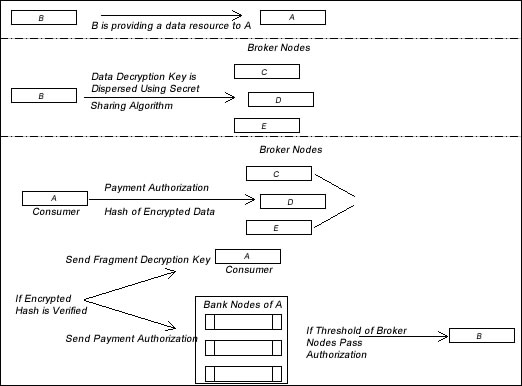
\includegraphics[height=85mm,width=65mm]{graphics/transaction.jpg}
  \caption{A transaction involving a distributed broker.}
  \end{center}
\end{figure}

Single broker solutions would entail P2P interactions being funneled through the lone broker leading to bottlenecks. The associated drawbacks in scaling, increased latencies due to queuing delays and the single point of failure that such a scheme constitutes are among the reasons favoring a distributed model being in place.

\subsection{Joining the network}
A node must contribute in some way before it will receive any currency.  One way a node could contribute is by providing content that other nodes are willing to provide currency to download.  A node could also contribute by performing administrative tasks such as acting as a broker or bank node. 

\subsection{Currency Management}
Currency is represented as discrete units.  There are two types of currency: data currency units and administrative currency units.  One or more data currency units can be used by a data consumer to obtain data from a data provider.  Administrative currency units are used to pay nodes for performing administrative tasks such as acting as a bank or broker.  A data currency unit can be converted into a number of administrative currency units.  Conversely administrative units from a sufficiently large number of different nodes can be converted into a data currency unit. A node can transfer a currency unit to another node by signing the currency unit along with an attached transfer authorization.

\subsection{Bank Nodes}
A set of bank nodes store the currency held by each node.  A node does not have control over the bank nodes assigned to it.  When a bank node receives a signed transfer authorization the sending bank node will remove the unit from its database and the receiving node will add the unit to its database.  A specific threshold of the bank nodes must agree to the presence of a currency unit for that unit to be considered valid.

\subsection{Currency Exchange}
\begin{enumerate}
\item Consumer requests data chunk from data provider
\item Provider sends the encrypted data chunk to the consumer
\item After receiving the encrypted data chunk the consumer calculates a hash of the encrypted data
\item The consumer then sends the hash along with the payment authorization to the broker
\item The broker compares the hash with the expected hash value.  If the hash is correct the broker will send the payment authorization to the provider and appropriate bank nodes and will send the decryption key to the consumer.  If the hash does not match the expected value the broker will notify the provider and consumer and destroy the payment authorization.
\end{enumerate}
In order for the broker to perform its duties it must have access to both the encrypted data hash and its fragment of the decryption key.  The data provider cannot be trusted to encrypt the data and provide this information to the broker.  If the broker has previously downloaded the data then it will have access to both the encrypted data hash and the decryption key otherwise a node can request its fragment of the decryption key from any node that has the complete decryption key.  Downloading newly added data carries with it an increased risk because there are no third-party brokers available.  Data consumers can use the number of available brokers as a criterion for determining how much to pay for a data transfer.  

\subsection{Storage}
Stuff here

\subsection{Automated transaction valuation based on reputation parameters}
Because of the risk of fraud inherent in peer-to-peer systems data consumers should attempt to use the most reputable data providers available.  It is expected that highly reputable data providers should receive more currency units per transaction than less reputable data providers.  Conversely data providers may charge less to more reputable data consumers.  The bank nodes of a node will track the following statistics:
\begin{itemize}
\item Number of complaints registered against the node
\item Number of complaints registered against the node for each file transferred
\item The number of data transactions performed by the node
\item The number of data transactions performed by the node for each file transferred
\item The number of administrative transactions performed by the node
\item The total number of each type of currency unit owned by the node
\item The average transfer rate for the node as reported by recent peers
\end{itemize}
Data consumers will also use the following information when determining how much currency to offer a data provider for a transfer:
\begin{itemize}
\item The number of nodes which can provide the data of interest
\item The number of brokers available for the data of interest
\item The number of nodes which are currently consuming the data of interest
\item A measure of the value the consumer places on obtaining the data
\end{itemize}
The state of the network is expected to be constantly changing.  Data consumers should be capable of automatically adjusting their valuations as network conditions change. 

\subsection{Distributed Hash Table}
Stuff here

%----------------------------------------------------------------------
% SECTION III: Simulation
%----------------------------------------------------------------------
\section{Simulation Experiments}
Statistics to collect:
\begin{itemize}
\item The number of invalid bytes received by cooperating consumers
\item The number of bytes received by cooperating consumers
\item The number of bytes sent by providers to consumers that did not pay
\item The number of bytes sent by providers
\item The number of band node requests
\item The number of broker node requests
\item The number of data transfer requests
\end{itemize}

\subsection{Simulation Framework}
Stuff here


\subsection{Simulation Results}
Stuff here

%----------------------------------------------------------------------
% SECTION IV: Conclusion
%----------------------------------------------------------------------
\section{Conclusion}
Milestone 3


% try out a theorem...
%\newtheorem{theorem}{Theorem}

%\begin{theorem}[Theorem name]
%  Consider the system ...
%\end{theorem}

%\begin{proof}
%  The proof is trivial.
%\end{proof}

% do the bibliography:
\bibliographystyle{IEEEbib}
\bibliography{cs598}

% where ``my-bibliography-file.bib'' is the name of the file with all the 
% BibTeX entries.

% do the biographies...
%\begin{biography}{Gregory L. Plett}
%  A bio with no face...
%\end{biography}

% If you want a picture with your biography, then specify the name of
% the postscript file in square brackets. That is, uncomment the
% following three lines and change the name of "face.ps" to the name of 
% your file.
%\begin{biography}[face.ps]{Gregory L. Plett}
%  A bio with a face...
%\end{biography}

%----------------------------------------------------------------------
% FIGURES
%----------------------------------------------------------------------
% There are many ways to include figures in the text. We will assume
% that the figure is some sort of EPS file.
%
% The outdated packages epsfig and psfig allow you to insert figures
% like: \psfig{filename.eps} These should really be done now using the
% \includegraphics{filename.eps} command.  
%
% i.e.,
%
% \includegraphics{file.eps}
%
% whenever you want to include the EPS file 'file.eps'. There are many
% options for the includegraphics command, and are outlined in the
% on-line documentation for the "graphics bundle". Using the options,
% you can specify the height, total height (height+depth), width, scale,
% angle, origin, bounding box "bb",view port, and can trim from around
% the sides of the figure. You can also force LaTeX to clip the EPS file
% to the bounding box in the file. I find that I often use the scale,
% trim and clip commands.
% 
% \includegraphics[scale=0.6,trim=0 0 0 0,clip=]{file.eps}
% 
% which magnifies the graphics by 0.6 (If I create a graphics for an
% overhead projector transparency, I find that a magnification of 0.6
% makes it look much better in a paper), trims 0 points off
% of the left, bottom, right and top, and clips the graphics. If the
% trim numbers are negative, space is added around the figure. This can
% be useful to help center the graphics, if the EPS file bounding box is
% not quite right.
% 
% To center the graphics,
% 
% \begin{center}
% \includegraphics...
% \end{center}
% 
% I have not yet written good documentation for this, but another 
% package which helps in figure management is the package ieeefig.sty,
% available at: http://www-isl.stanford.edu/people/glp/ieee.shtml
% Specify:
% 
%\usepackage{ieeefig} 
% 
% in the preamble, and whenever you want a figure,
% 
%\figdef{filename}
% 
% where, filename.tex is a LaTeX file which defines what the figure is.
% It may be as simple as
% 
% \inserteps{filename.eps}
%
% or
% \inserteps[includegraphics options]{filename.eps}
% 
% or may be a very complicated LaTeX file. 

\end{document}
